\providecommand{\home}{../../../..}
\documentclass[\home/main.tex]{subfiles}
\usetikzlibrary[arrows,snakes,backgrounds]
\usetikzlibrary{calc,positioning}

\begin{document}

% ===================
%     COMPLETE FIG
% ===================

\begin{tikzpicture}
    \def\picMinWidth{5cm}
    \def\picMinHeight{4.0cm}

    \tikzset{
        block/.append style={node distance=35mm,minimum width=3.5cm},
        picture/.style={block, node distance=6cm, fill=white, draw=white,minimum width=\picMinWidth, minimum height=\picMinHeight, text width=\picMinWidth,},
        preSpacedDash/.style={preSpaced, dashed,draw=black!50, thin},
        annot/.style={text width=4em, text centered},
    }

    \node[block] (obs) {Isolate};
    \node[picture] (obs_pic) [right of=obs] {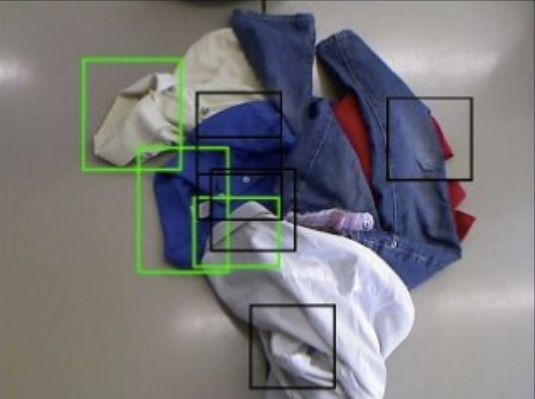
\includegraphics[width=\picMinWidth, height=\picMinHeight]{\home/chapters/02-sota/figures/fig-folding-pipeline-subtasks/isolate}}
    edge[preSpacedDash] node[midway,above=0.5pt,]{\tiny{\textcolor{black!50}{example (\textbf{a})}}} (obs);

    \node[block] (state) [below of=obs] {Unfold}
    edge[preSpacedArrow] node[midway,left,text width=10mm,align=left,text=gray,font=\tiny\linespread{0.1}\selectfont]{single\\clothing\\item} (obs);
    \node[picture] (state_pic) [right of=state] {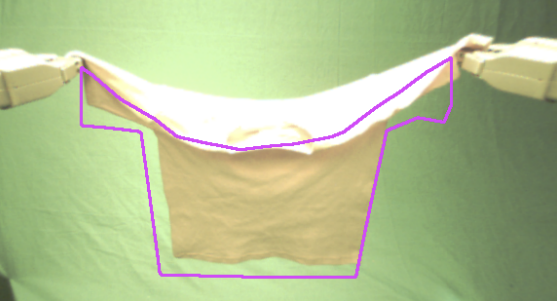
\includegraphics[width=\picMinWidth, height=\picMinHeight]{\home/chapters/02-sota/figures/fig-folding-pipeline-subtasks/unfolding}}
    edge[preSpacedDash] node[midway,above=0.5pt,]{\tiny{\textcolor{black!50}{example (\textbf{b})}}} (state);

    \node[block] (modeling) [below of=state,align=center] {Flatten}
    edge[preSpacedArrow] node[midway,left,text width=10mm,align=left,text=gray,font=\tiny\linespread{0.1}\selectfont]{unfolded\\clothing\\item} (state);
    \node[picture] (modeling_pic) [right of=modeling] {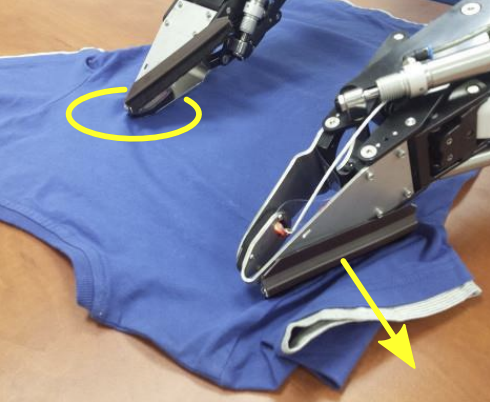
\includegraphics[width=\picMinWidth, height=\picMinHeight]{\home/chapters/02-sota/figures/fig-folding-pipeline-subtasks/flattening}}
    edge[preSpacedDash] node[midway,above=0.5pt,]{\tiny{\textcolor{black!50}{example (\textbf{c})}}} (modeling);

    \node[block] (planning) [below of=modeling] {Folding}
    edge[preSpacedArrow] node[midway,left,text width=10mm,align=left,text=gray,font=\tiny\linespread{0.1}\selectfont]{wrinkle-free\\clothing\\item} (modeling);
    \node[picture] (planning_pic) [right of=planning] {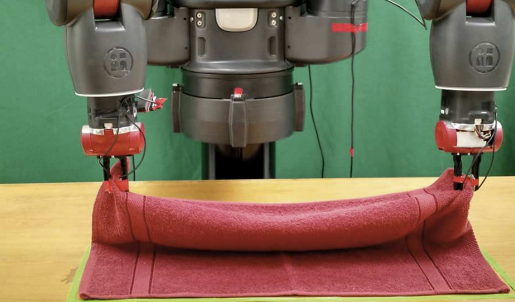
\includegraphics[width=\picMinWidth, height=\picMinHeight]{\home/chapters/02-sota/figures/fig-folding-pipeline-subtasks/folding}}
    edge[preSpacedDash]  node[midway,above=0.5pt,]{\tiny{\textcolor{black!50}{example (\textbf{d})}}} (planning);

    \node[block] (control) [below of=planning] {Stacking}
    edge[preSpacedArrow] node[midway,left,text width=10mm,align=left,text=gray,font=\tiny\linespread{0.1}\selectfont]{folded\\clothing\\item} (planning);
    \node[picture] (control_pic) [right of=control] {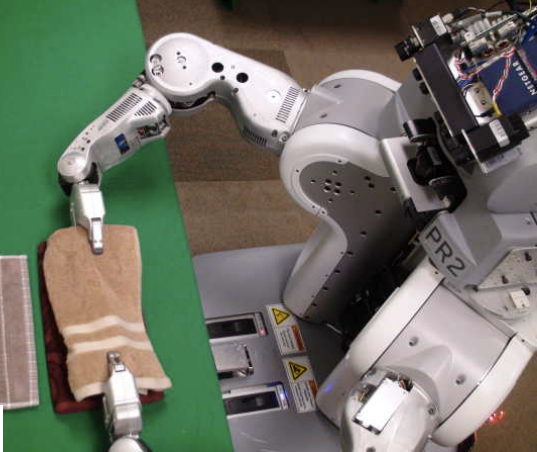
\includegraphics[width=\picMinWidth, height=\picMinHeight]{\home/chapters/02-sota/figures/fig-folding-pipeline-subtasks/stacking}}
    edge[preSpacedDash] node[midway,above=0.5pt,]{\tiny{\textcolor{black!50}{example (\textbf{e})}}} (control);

\end{tikzpicture}

\end{document}
